% !TEX encoding = UTF-8
% !TEX TS-program = pdflatex
% !TEX root = ../Tesi.tex
% !TEX spellcheck = it-IT

%************************************************
\chapter{Modello di design}
\label{cap:modello-di-design}
%************************************************

\section{Diagramma delle classi}
	Il raffinamento del modello delle classi di dominio avviene attraverso il modello di design suddividendo tutte le classi del progetto in tre categorie:
	\begin{enumerate}
		
		\item
		Classi Boundary;
		
		\item
		Classi Control;
		
		\item
		Classi Entity.
		
	\end{enumerate}
	Di seguito vengono presentate le categorie sopracitate.

	\subsection{Classi Boundary}
	Sono le classi che si interfacciano con l'utente.
	
	Le classi boundary rappresentano un punto di interfaciamento bidirezionale tra gli attori ed il sistema.
	
	Nel caso dell'applicazione web, queste sono le singole pagine JSP che in fase di compilazione vengono convertite in Servlet (classi Java che estendono la classe \texttt{HTTPServlet}).
	
	Gli attori sono: Admin (amministratore), Arbitro, Gestore (gestore di una squadra) e Guest (utente pubblico).
	
	Si procede con l'elenco delle classi Boundary:
	
	\subsubsection*{Admin:}
	
		\begin{itemize}
			\item Calendario.jsp
			\item dettagliTorneo.jsp
			\item dettagliUtente.jsp
			\item homeA.jsp
			\item newReferto.jsp
			\item newTorneo.jsp
			\item referti.jsp
			\item refertiView.jsp
			\item selezionaSquadre.jsp
			\item tornei.jsp
			\item utenti.jsp	
		\end{itemize}
	
	\subsubsection*{Arbitro:}
	
	\begin{itemize}
		\item dettagliReferto.jsp
		\item homeR.jsp
		\item myReferti.jsp
		\item referti.jsp	
	\end{itemize}
	
	\subsubsection*{Gestore:}
	
	\begin{itemize}
		\item dettagliGiocatore.jsp
		\item giocatori.jsp
		\item homeG.jsp
		\item newFormazione.jsp
		\item sceltaGiocatori.jsp
		\item squadre.jsp	
	\end{itemize}
	
	\subsubsection*{Guest:}
	
	\begin{itemize}
		\item listaGiocatori.jsp
		\item listaSquadre.jsp
		\item listaTornei.jsp
		\item vediGiocatore.jsp
		\item vediReferto.jsp
		\item vediSquadra.jsp
		\item vediTorneo.jsp	
	\end{itemize}

	\subsubsection*{Tutti gli utenti:}
	
	\begin{itemize}
		\item ErrorPage.jsp
		\item login.jsp
		\item home.jsp	
	\end{itemize}
	
	\subsection{Classi Control}
	Sono le classi che validano le interazioni dell'utente e si interfacciano con la base dati.
	
	Queste classi incapsulano la logica applicativa dei casi d'uso sopra elencati. Il compito di queste classi è quello di coordinare il lavoro svolto da istanze delle classi \emph{Boundary} ed \emph{Entity}.
	
	Nel caso dell'applicazione web, queste sono le classi della \emph{Business Logic}, i \emph{Services} associati e le classi che governano il flusso delle conversazioni.
	
	\subsubsection*{Package bflows:}
	Il package \texttt{bflows} (acronimo di \emph{BusinessFlows}) si occupa del controllo del flusso delle conversazioni.
	Le classi di questo package usano le classi del package \texttt{blogics} (acronimo di \emph{BusinessLogics}) che si occupano di mappare l'oggetto del database e di fornire i servizi interessati dalla conversazione medesima.
	Si nota che una conversazione può avere più classi \emph{Boundary} associate.
	
	\subsubsection*{Package blogics:}
	Il package \texttt{blogics} si occupa di rendere disponibili tutte le funzioni e i servizi che l'applicazione web può offrire.
	I servizi presenti in questo package non sono vincolati in alcun modo a particolari interfacce o a determinate conversazioni, ma possono essere utilizzate in più contesti.
	
	\subsubsection*{Package service:}
	Le classi contenute in questo package sono classi di servizio. Infatti si può notare che il costruttore di tali classi è privato e che tutti i metodi delle classi sono statici.
	
	In particolare si osserva nella classe \texttt{DBService.java} l'implementazione del pattern \emph{Singleton} che gestisce la connessione al database.
	
	\subparagraph{databaseservice}
	Le classi contenute in questa sottocartella della classe services, permettono di gestire la connessione al database.
	
	%
	% Figura: classi della cartella databaseservice
	%
	\begin{figure}[h]
		\centering
		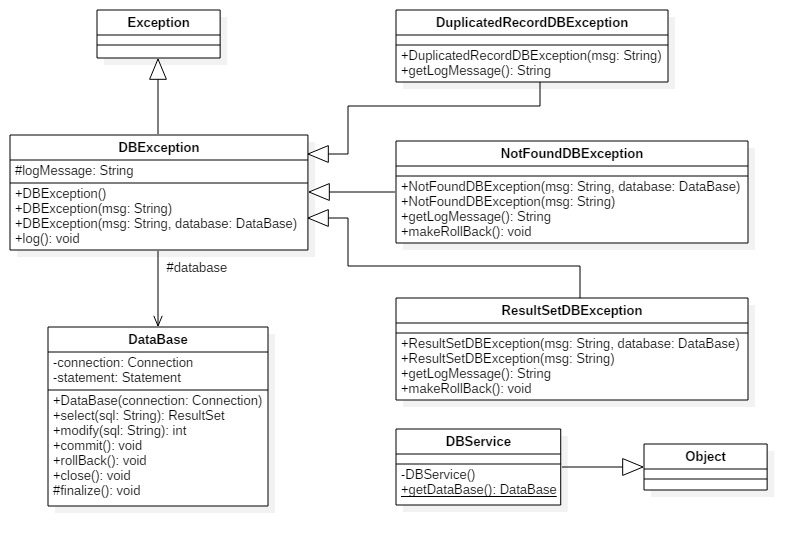
\includegraphics[width=0.4\textwidth]
		{immagini/c-databaseservice}
		
		\caption{Classi della sotto-cartella databaseservice}
	\end{figure}
	
	
	\subparagraph{errorservice}
	Le classi contenute in questa sottocartella della classe services, permettono di gestire gli errori che si possono generare durante l'esecuzione dell'applicazione.
	
	%
	% Figura: classi della cartella errorservice
	%
	\begin{figure}[h]
		\centering
		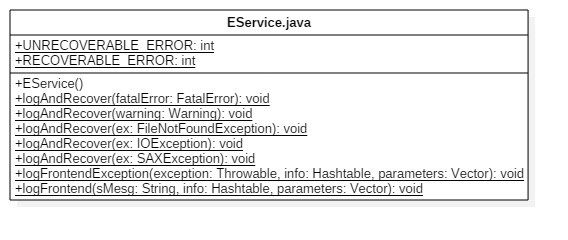
\includegraphics[width=0.4\textwidth]
		{immagini/c-errorservice}
		
		\caption{Classi della sotto-cartella errorservice}
	\end{figure}
	
	
	\subparagraph{logservice}
	Le classi contenute in questa sottocartella della classe services, permettono di scrivere i messaggi di errore in uno specifico file denominato \emph{log}.
	
	%
	% Figura: classi della cartella logservice
	%
	\begin{figure}[h]
		\centering
		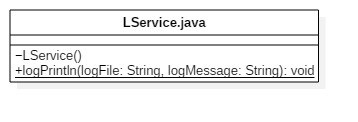
\includegraphics[width=0.4\textwidth]
		{immagini/c-logservice}
		
		\caption{Classi della sotto-cartella logservice}
	\end{figure}
	
	
	\subparagraph{sessionservice}
	La classe contenute in questa sottocartella della classe services, permette di gestire la sessione tramite il protocollo \texttt{HTTP}.
	
	%
	% Figura: classi della cartella sessionservice
	%
	\begin{figure}[h]
		\centering
		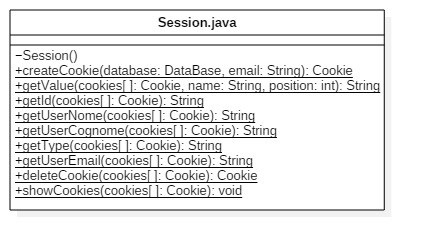
\includegraphics[width=0.4\textwidth]
		{immagini/c-sessionservice}
		
		\caption{Classi della sotto-cartella sessionservice}
	\end{figure}
	
	
	\clearpage
	
	%
	% Figura: classi del package bflows
	%
	\begin{figure}[h]
		\centering
		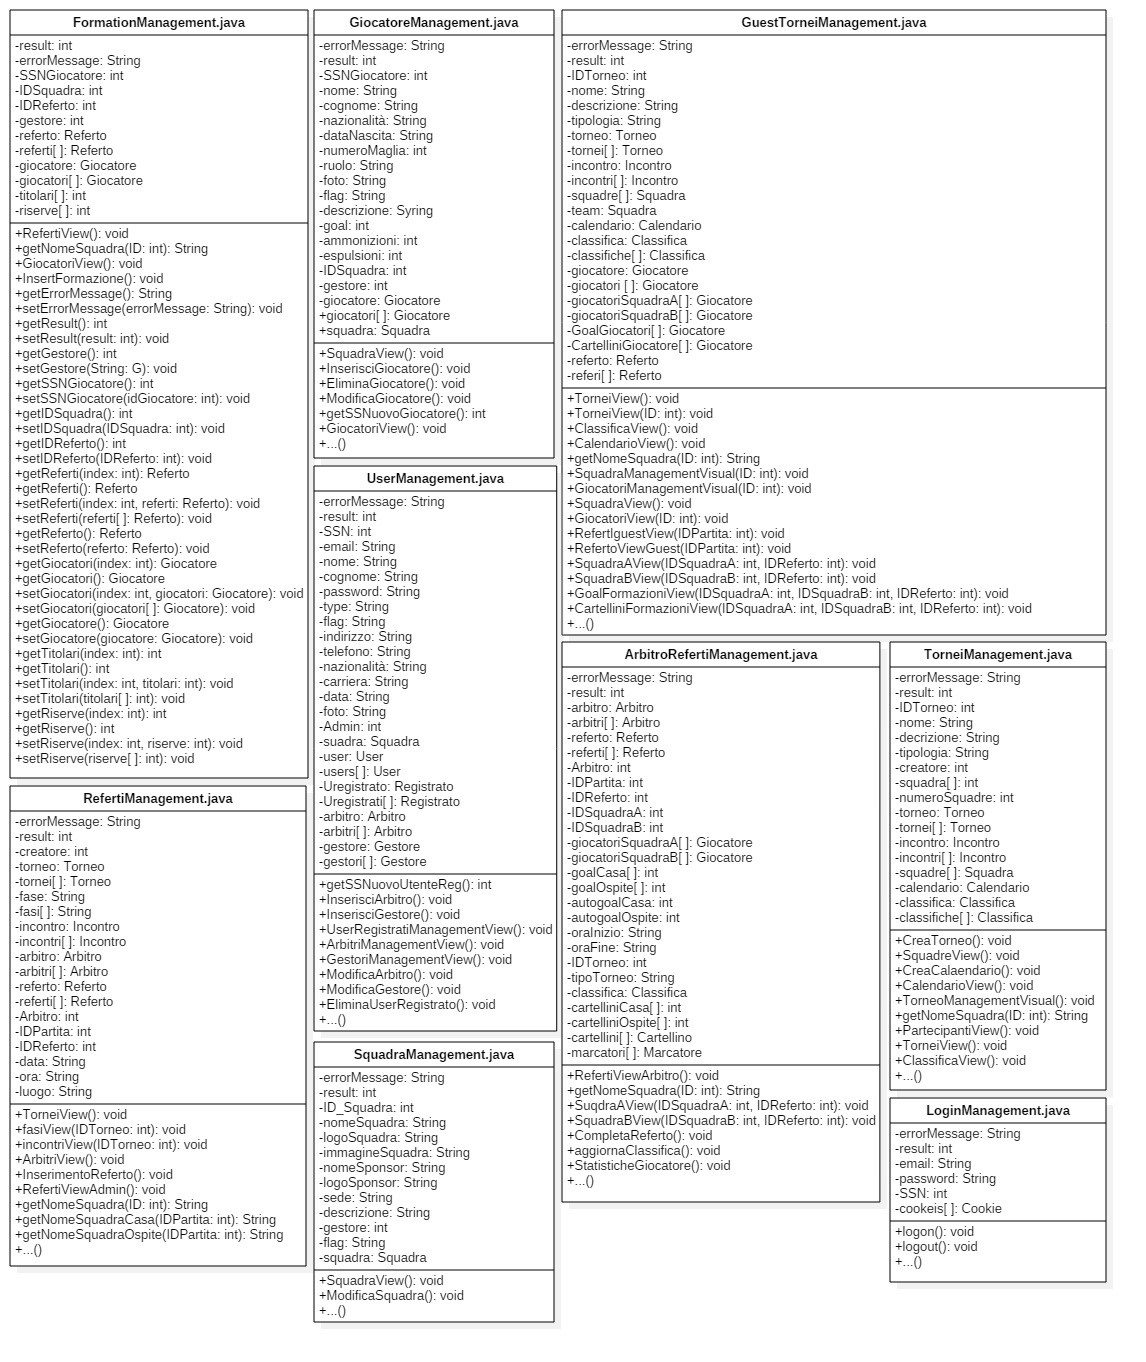
\includegraphics[width=1\textwidth]
		{immagini/c-bflows}
		
		\caption{Classi del package bflows}
	\end{figure}
	
	\subsubsection*{N.B.}
	Il simbolo $+...()$ sta indica tutti i metodi getter e setter utili per far funzionare correttamente l'applicazione. Si è scelto di non inserirli per non aggiungere ulteriore complessità ai diagrammi.
	
	\clearpage
	
	%
	% Figura: classi del package blogics
	%
	\begin{figure}[h]
		\centering
		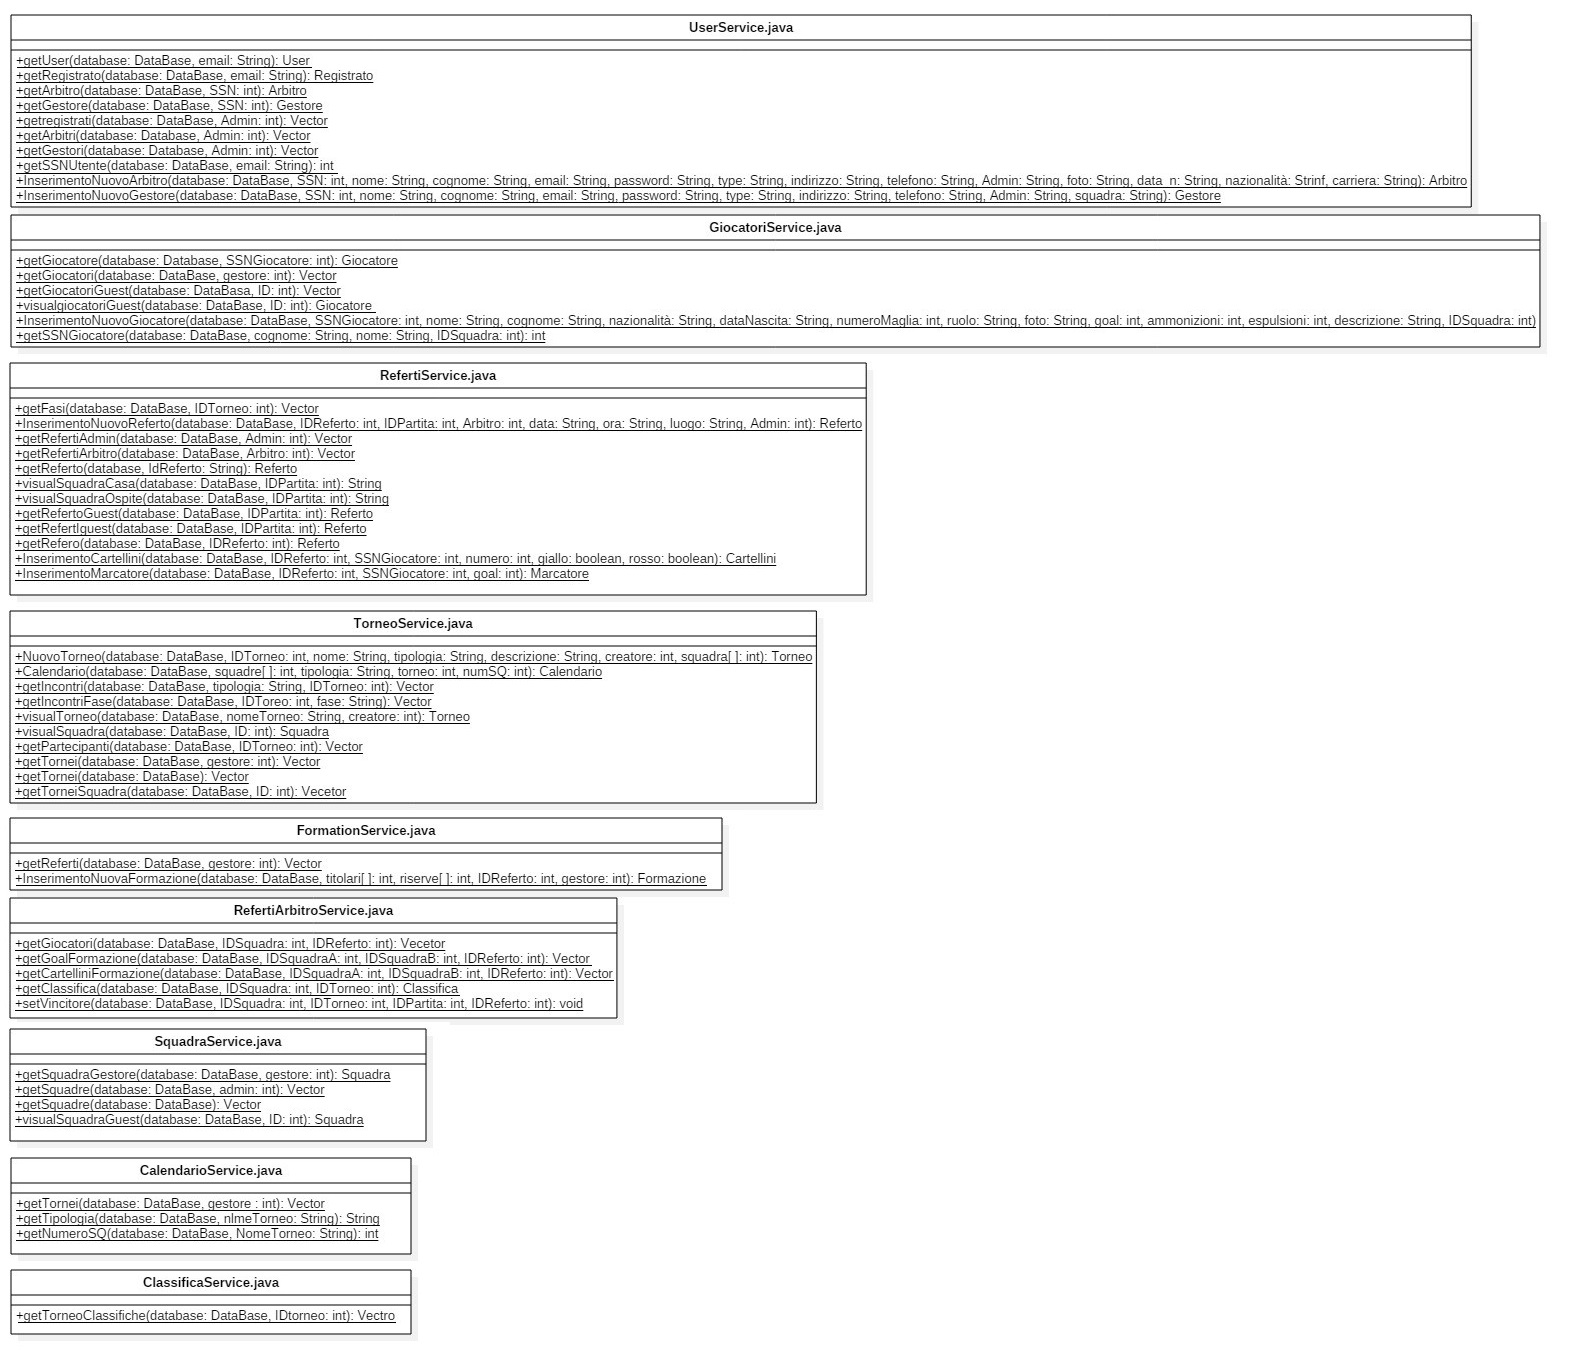
\includegraphics[width=1\textwidth]
		{immagini/c-service-blogics}
		
		\caption{Classi service del package blogics}
	\end{figure}
	
	\clearpage
	
	\subsection{Classi Entity}
	Sono le classi che mappano la struttura della base dati.
	
	Le classi Entity modellano le informazioni gestite dal sistema e formalizzano la struttura logica dei dati, in modo da isolare i dettagli della memorizzazione dei dati e di limitare l'impatto di eventuali modifiche alla struttura del database.
	
	Nel caso dell'applicazione web, queste sono le classi della \emph{Business Logic} che implementano i metodi setter, getter e i costruttori per creare l'oggetto mediante passaggio di dati di tipo primitivo od oggetti quali \texttt{RecordSet}.
	
	La figura \vref{c-blogics} rappresenta le classi di questo tipo.
	
	%
	% Figura: classi del package blogics
	%
	\begin{figure}[h]
		\centering
		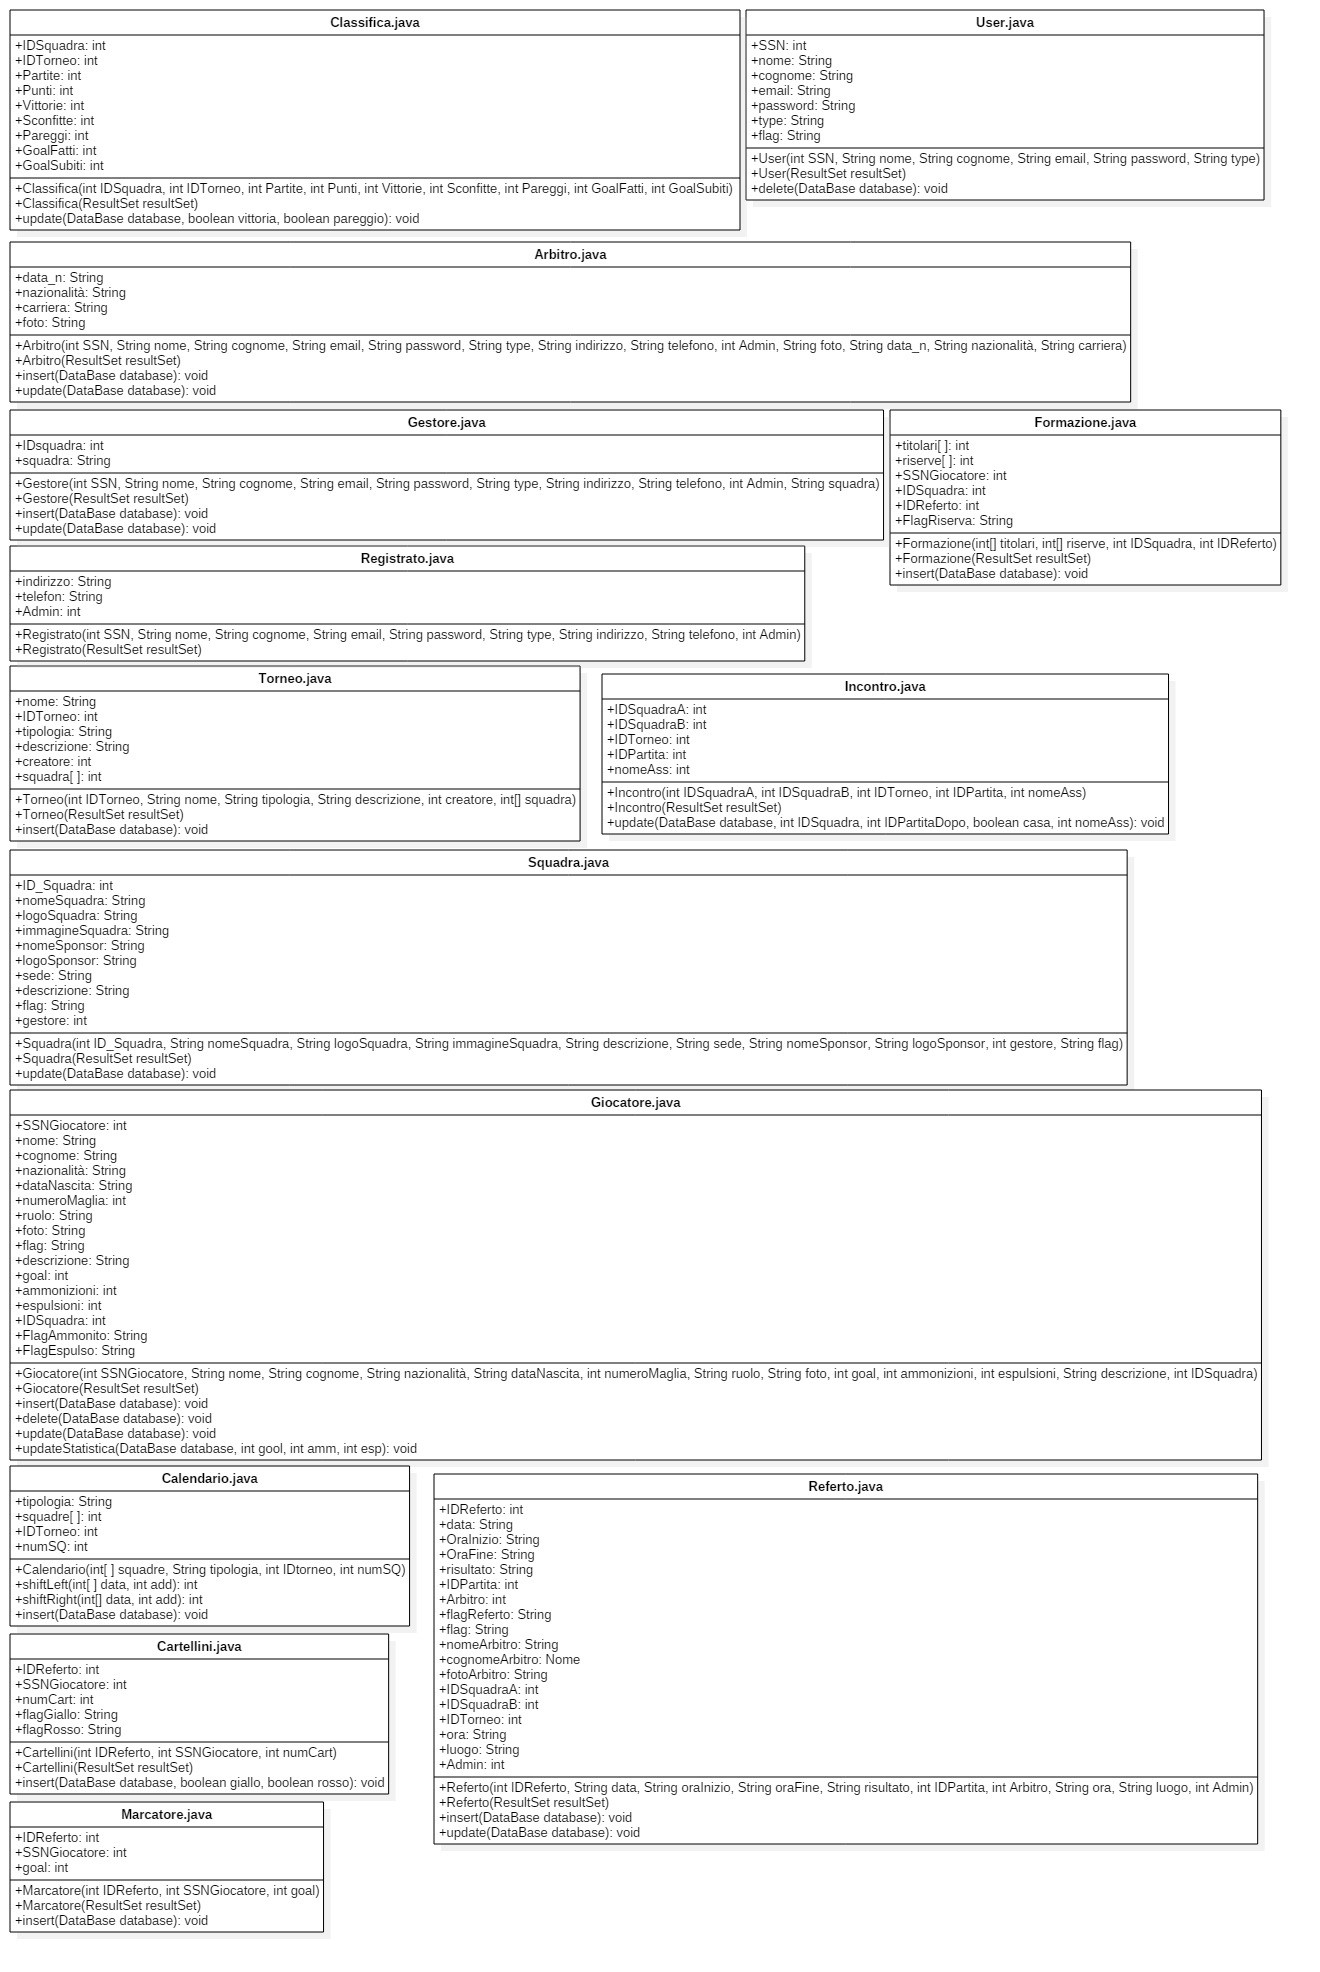
\includegraphics[width=1\textwidth]
		{immagini/c-blogics}
		
		\caption{Classi del package blogics}
		\label{c-blogics}
	\end{figure}

\clearpage

\section{Diagrammi di sequenza}
Si riporta a titolo di esempio un Sequence Diagram relativo alla creazione della formazione di una squadra per una partita.

Il gestore di una determinata squadra si occupa della creazione della formazione per una specifica partita di un torneo.

%
% Figura: diagramma di sequenza
%
\begin{figure}[h]
	\centering
	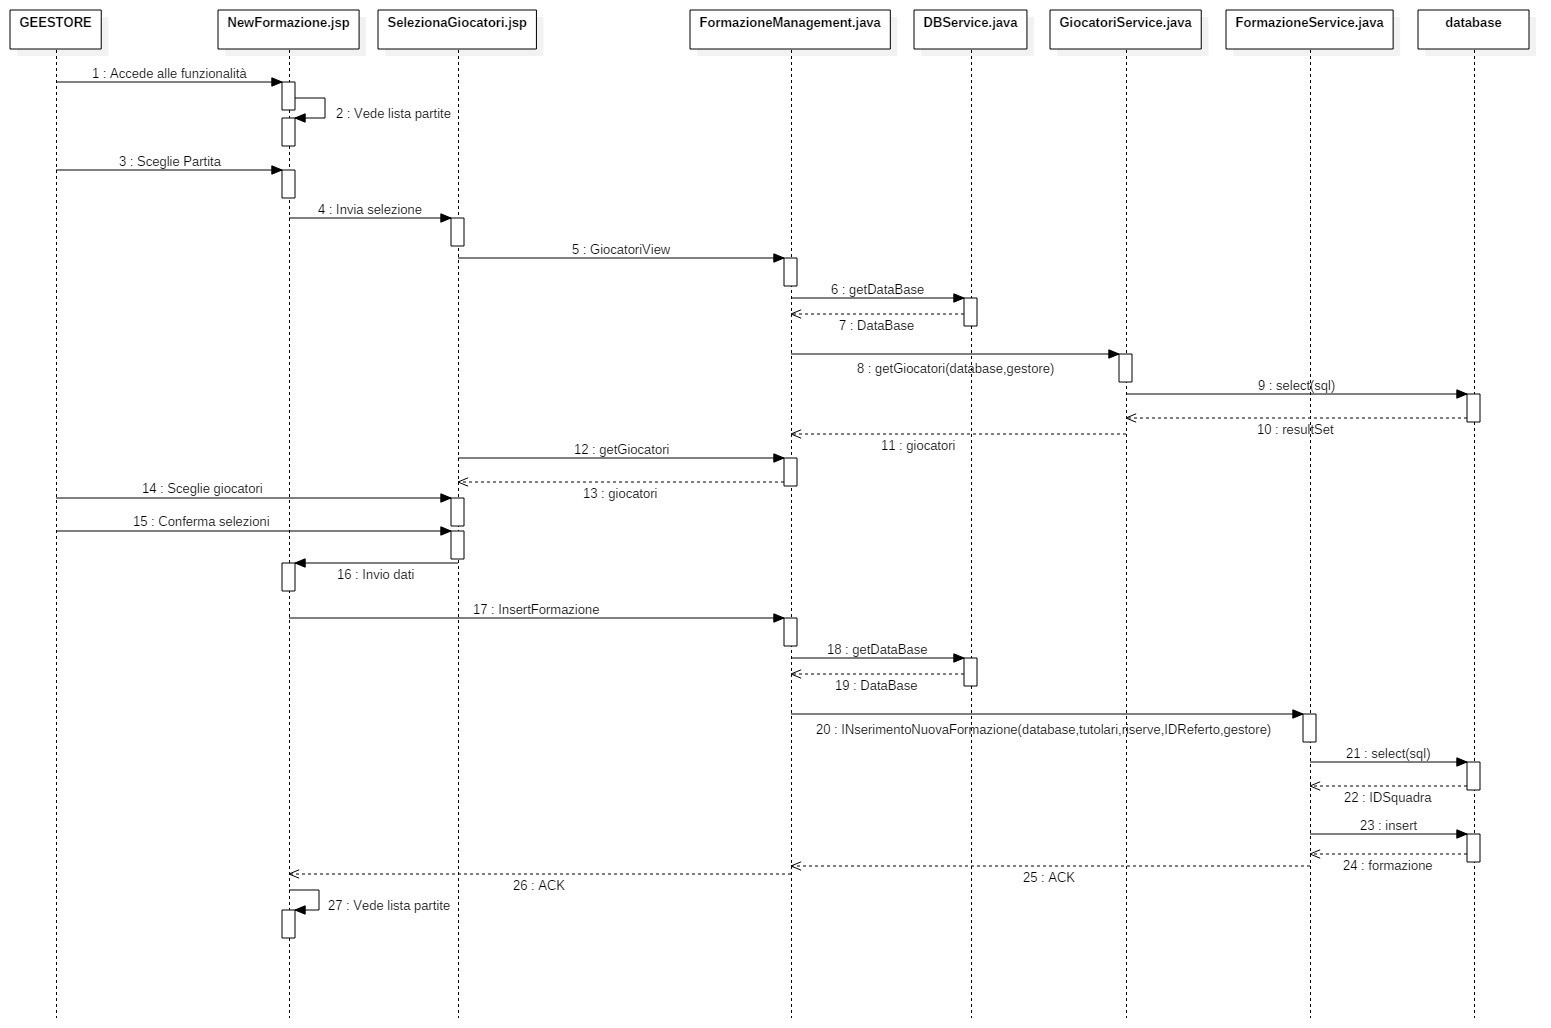
\includegraphics[width=1\textwidth]
	{immagini/sd-partita}
	
	\caption{Diagramma di sequenza della creazione della formazione di una squadra}
\end{figure}